\documentclass[handout]{beamer}


\usepackage[swedish]{babel}
\ifluatex
    \usepackage{euler}
    \usepackage{fontspec}
\else
    \usepackage[utf8]{inputenc}
	\usepackage[T1]{fontenc}
    \usepackage{euler}
\fi
\usepackage{tikz}
\usepackage[nice]{units}

\usepackage[iso, swedish]{isodate}
\usepackage{multimedia}
\definecolor{links}{HTML}{0000FF}
\hypersetup{colorlinks,linkcolor=,urlcolor=links}

\usetikzlibrary{calc,shapes.callouts,shapes.arrows}

\usetheme{Warsaw}
\useoutertheme[subsection=false]{miniframes}

\setbeamercolor{normal text}{fg=black,bg=white}
\setbeamercolor{structure}{fg=black}

\setbeamercolor{alerted text}{fg=red!85!black}

\setbeamercolor{item projected}{use=item,fg=black,bg=item.fg!35}

\setbeamercolor{palette primary}{bg=black!90, fg=white!90}
\setbeamercolor{palette secondary}{bg=black!80,fg=white}
\setbeamercolor{palette tertiary}{bg=black!90,fg=white}
\setbeamercolor{palette quaternary}{fg=red, bg=red}
% \setbeamercolor{lower separation line head}{bg=black!60}
% \setbeamerfont{headline}{size=\fontsize{7}{11}}

\setbeamercolor{framesubtitle}{fg=black}
\setbeamercolor{frametitle}{fg=white, bg=black!80}

\setbeamercolor{block title}{parent=structure,bg=black!60}
\setbeamercolor{block body}{fg=black,bg=black!10}
\setbeamercolor{block title alerted}{parent=alerted text,bg=black!15}
\setbeamercolor{block title example}{parent=example text,bg=black!15}



\newcommand{\explain}[2]{
        \tikz[remember picture,baseline]{\node[anchor=base,inner sep=0,outer sep=0]%
        (#1) {#1};\node[overlay,rectangle callout,fill=orange!40]
        at ($(#1.north)+(-.5cm,0.8cm)$) {\small #2};}%
    }%


\newcommand{\entry}[2][]{%
\item #2 \ifthenelse{\isempty{#1}}{}{\hfill #1}
}

\newcommand{\descr}[3][]{%
\item \textbf{#2} \ifthenelse{\isempty{#1}}{}{\hfill #1}
\ifthenelse{\isempty{#3}}{}{\par #3}
}

\defbeamertemplate*{footline}{shadow theme}{%
\leavevmode%
\hbox{\begin{beamercolorbox}[wd=.5\paperwidth,ht=2.5ex,dp=1.125ex,leftskip=.3cm plus1fil,rightskip=.3cm]{author in head/foot}%
    \usebeamerfont{author in head/foot}\hfill\insertshortauthor
\end{beamercolorbox}%

\begin{beamercolorbox}[wd=.5\paperwidth,ht=2.5ex,dp=1.125ex,leftskip=.3cm,rightskip=.3cm plus1fil]{title in head/foot}%
    \usebeamerfont{title in head/foot}\insertshorttitle\hfill%
\insertframenumber\,/\,\inserttotalframenumber
\end{beamercolorbox}}%
\vskip0pt%
}

\usetikzlibrary{shapes,arrows}
\tikzstyle{block} = [rectangle, draw, fill=red!20,
    text width=7em, text centered, rounded corners, minimum height=4em]
\tikzstyle{blockfade} = [rectangle, draw, fill=red!5,
    text width=7em, text centered, rounded corners, minimum height=4em]

\tikzstyle{blockfat} = [rectangle, draw, fill=red!70,
    text width=7em, text centered, rounded corners, minimum height=4em]

\tikzstyle{line} = [draw, -latex']
\tikzstyle{cloud} = [draw, ellipse,fill=red!20, node distance=3cm,
    minimum height=2em]


%\addtobeamertemplate{frametitle}{\let\insertframetitle%\insertsubsectionhead}{}
%\makeatletter
%  \CheckCommand*\beamer@checkframetitle{\@ifnextchar\bgroup%\beamer@inlineframetitle{}}
%  \renewcommand*\beamer@checkframetitle{\global\let\beamer@frametitle\relax\@ifnextchar\bgroup\beamer@inlineframetitle{}}
%\makeatother

\title{Design av Robothand}
\date{2013-03-13}
\author{Håkansson, Larsson, Olsson, Kvist, Soureh, Öjeling}


\begin{document}

\begin{frame}[plain]
\begin{columns}
\begin{column}{0.4\textwidth}

{\large \bfseries Design av Robothand} \\
2013-06-04
\par
\medskip
\hline
\vspace{1cm}


Christopher Håkansson \\
Emil Kvist \\
Christoffer Öjeling

\end{column}

\begin{column}{0.6\textwidth}
\includegraphics[height=\textheight]{img/overgrip}
\end{column}

\end{columns}
\end{frame}


% \begin{frame}
% \movie{placeholder box}{filmer/Redovisning.m4v}
% \end{frame}

\begin{frame}
\tableofcontents %Listan blir ihoptryckt när bilden läggs till...
% \vspace{-5cm}
% \begin{center}
% \hspace*{5cm}\includegraphics[height=0.9\textheight]{img/overgrip}
% \end{center}
\end{frame}

\section{Inledning}


\begin{frame}
\frametitle{Cutkoskys handmodeller}
\includegraphics[width=0.85\textwidth]{img/cutkoskys_handmodeller}
\end{frame}

\begin{frame}
\frametitle{Cutkoskys handmodeller}
\includegraphics[width=0.85\textwidth]{img/cutkoskyscadgrepp}
\end{frame}

\begin{frame}
\frametitle{Flödesschema}
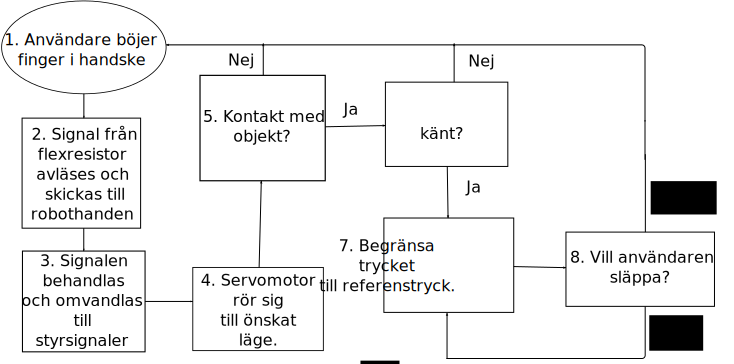
\includegraphics[width=\textwidth]{img/flodesschema}
\end{frame}

\section{Robothanden}
\begin{frame}
\frametitle{Robothand}
\includegraphics[width=\textwidth]{img/hand}
\end{frame}
\begin{frame}
\frametitle{Finger}
\includegraphics[width=\textwidth]{img/fingerbild}
\end{frame}
\begin{frame}
\frametitle{Stag och sena}
\includegraphics[width=\textwidth]{img/stagsenor}
\end{frame}
\begin{frame}
\frametitle{Fingertoppar}
\includegraphics[width=0.5\textwidth]{img/sensor}
\includegraphics[width=0.55\textwidth]{img/trycksensor}
\end{frame}

\section{Styrhandsken}
\begin{frame}
\frametitle{Styrhandsken}
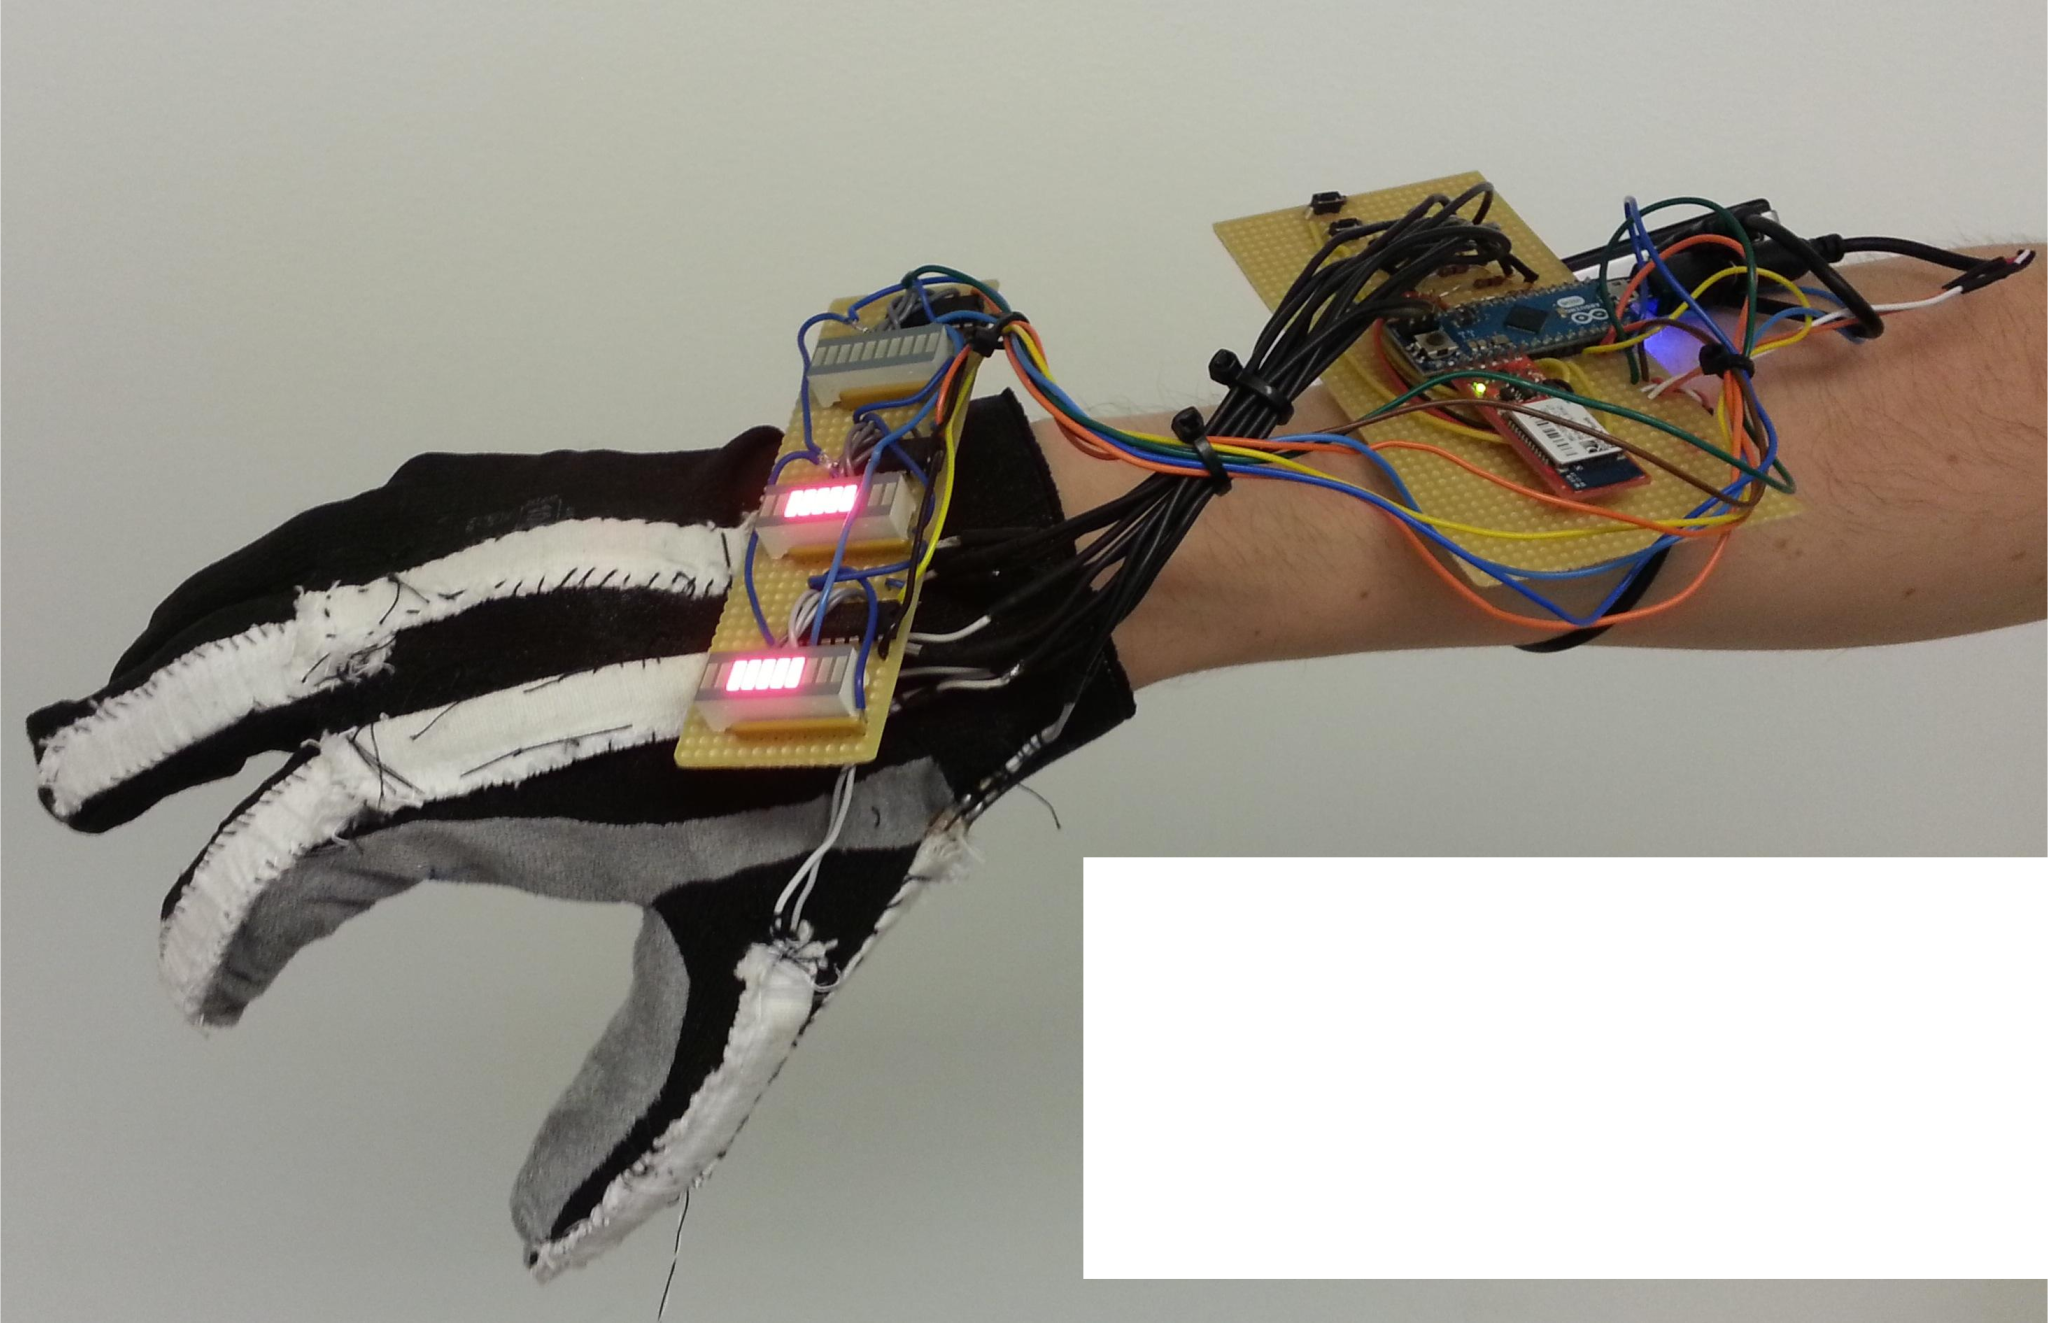
\includegraphics[width=\textwidth]{img/styrhandskediod}
\end{frame}

\section{Signalbehandling}
\subsection{Styrhandsken}
\begin{frame}
\frametitle{Signalens väg för styrhandsken}
\footnotesize
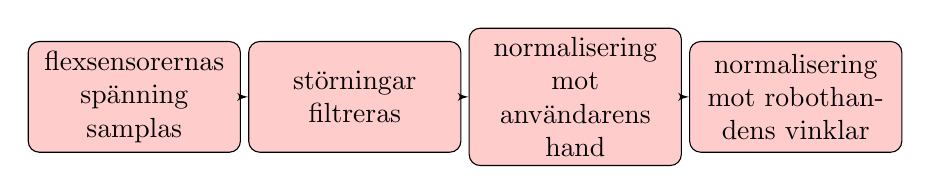
\begin{tikzpicture}[node distance = 2.8cm, auto]
    \node [block] (sampling) {flexsensorernas spänning samplas};
    \node [block, right of=sampling] (filter) {störningar filtreras};
    \node [block, right of=filter] (norm1) {normalisering mot användarens hand};
    \node [block, right of=norm1] (norm2) {normalisering mot robothandens vinklar};

    \path [line] (sampling) -- (filter);
    \path [line] (filter) -- (norm1);
    \path [line] (norm1) -- (norm2);
\end{tikzpicture}
\end{frame}
\subsection{Robothanden}
\begin{frame}
\frametitle{Signalens väg för robothanden}
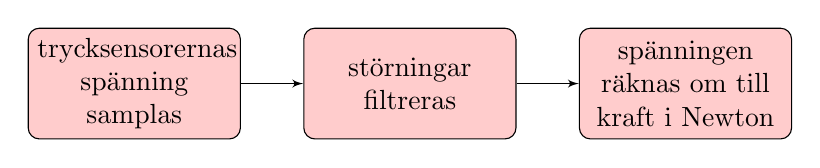
\begin{tikzpicture}[node distance = 3.5cm, auto]
    \node [block] (sampling) {trycksensorernas spänning samplas};
    \node [block, right of=sampling] (filter) {störningar filtreras};
    \node [block, right of=filter] (norm1) {spänningen räknas om till kraft i Newton};

    \path [line] (sampling) -- (filter);
    \path [line] (filter) -- (norm1);
 \end{tikzpicture}
\end{frame}


\section{Objektidentifiering}
\begin{frame}
\frametitle{Servovinklar}
\includegraphics[width=\textwidth]{img/servo_vinklar}
\end{frame}
\begin{frame}
\frametitle{Modell av handen}
\includegraphics[width=\textwidth]{img/matlab_modell}
\end{frame}
\begin{frame}
\frametitle{Jämförelse mot verkliga värden}
\includegraphics[width=\textwidth]{img/obj_id_matlab2-eps-converted-to}
\end{frame}

\section{Tryckbegränsning}
\begin{frame}
\frametitle{Ett1}
\includegraphics[width=\textwidth]{img/masterplot}
\end{frame}



\end{document}
